\documentclass[oneside,final,14pt,a4paper]{extreport}

\usepackage{tempora} % Times New Roman alike font  

\usepackage{vmargin}
\setpapersize{A4}
\setmarginsrb{2.5cm}{2.2cm}{2.2cm}{2.2cm}{0pt}{10mm}{0pt}{13mm}
\usepackage{setspace}
\setstretch{1.5}
\usepackage{indentfirst}
\parindent=1.25cm

%%%%% ADDED TO SUPPORT TT BOLD FACES %%%%
\DeclareFontShape{OT1}{cmtt}{bx}{n}{<5><6><7><8><9><10><10.95><12><14.4><17.28><20.74><24.88>cmttb10}{}
\renewcommand{\ttdefault}{pcr}
%%%%% END %%%%%%%%%%%%%%%%%%%%%%%%%%%%%%% 

\usepackage{atbegshi,picture}
\usepackage[T1,T2A]{fontenc}
\usepackage[utf8]{inputenc}

\usepackage[english]{babel}
\usepackage[backend=biber,style=ieee,autocite=inline]{biblatex}
\bibliography{ref.bib}
\DefineBibliographyStrings{english}{%
  bibliography = {References},}
\usepackage{blindtext}

\usepackage{pdfpages}
\newenvironment{bottompar}{\par\vspace*{\fill}}{\clearpage}
\usepackage{amsmath,amsfonts}
\usepackage{url}
\usepackage{amsthm}
\newtheorem{theorem}{Theorem}
\newtheorem{corollary}{Corollary}
\newtheorem{lemma}{Lemma}
\newtheorem{proposition}{Proposition}
\theoremstyle{definition}
\newtheorem{definition}{Definition}
\theoremstyle{remark}
\newtheorem*{remark}{Remark}
\theoremstyle{remark}
\newtheorem*{example}{Example}

\usepackage{float}
\usepackage{graphicx}
\graphicspath{{figs/}} %path to images
\usepackage{array}
\usepackage{multirow,array}
\usepackage{caption}
\usepackage{subcaption}
\usepackage{hyperref}
\hypersetup{colorlinks=true, allcolors=black, citecolor=black}
\usepackage{paralist}
\usepackage{listings}
\usepackage{zed-csp}
\usepackage{fancyhdr}
\usepackage{csquotes}
\usepackage{color}
% \usepackage{anyfontsize}
% \usepackage{mathptmx}
% \usepackage{t1enc}

\usepackage{chngcntr}
\usepackage{upgreek} 
\usepackage{bm}
\usepackage{hyperref}
\usepackage{booktabs}
\usepackage{multirow}
\usepackage{longtable}

\usepackage[font=singlespacing, labelfont=bf]{caption}
%Hints
\newcommand\pic[1]{(Fig. \ref{#1})} %Ref on figure
\newcommand\tab[1]{(Tab. \ref{#1})} %Ref on table

\setlength{\headheight}{32.0976pt}
\usepackage{enumitem}
\newlist{inlinelist}{enumerate*}{1}
\setlist*[inlinelist,1]{%
  label=(\arabic*),
}

% \setcounter{secnumdepth}{4}
\captionsetup[table]{labelfont={normalfont}, name={TABLE}, labelsep={newline}}
\setlength{\parindent}{2em} 
\DeclareCaptionLabelSeparator{figSep}{.\quad}
\captionsetup[figure]{labelfont={normalfont}, name={Fig.}, labelsep=period}
% \counterwithin{figure}{chapter}

\usepackage{titlesec}
\titleformat{\section}[hang]{\fontsize{20}{24}\selectfont\filcenter}{\Roman{section}}{1em}{}
\titleformat{\subsection}[hang]{\itshape}{\Alph{subsection}.}{1em}{}[]
\titleformat{\subsubsection}[runin]{\itshape}{\arabic{subsubsection})}{1em}{}[$:$]
\titlespacing{\subsubsection}{1em}{1em}{1em}
\titleformat{\paragraph}[runin]{\itshape}{\alph{paragraph})}{1em}{}[$:$\quad]
\titlespacing{\paragraph}{2em}{1em}{1em}

\usepackage{placeins} % for \FloatBarrier
\usepackage{algpseudocode}
\pagestyle{fancyplain}

% remember section title
\renewcommand{\chaptermark}[1]%
	{\markboth{\chaptername~\thechapter~--~#1}{}}

% subsection number and title
\renewcommand{\sectionmark}[1]%
	{\markright{\thesection\ #1}}

\rhead[\fancyplain{}{\bf\leftmark}]%
      {\fancyplain{}{\bf\thepage}}
\lhead[\fancyplain{}{\bf\thepage}]%
      {\fancyplain{}{\bf\rightmark}}
\cfoot{} %bfseries


\newcommand{\dedication}[1]
   {\thispagestyle{empty}
     
   \begin{flushleft}\raggedleft #1\end{flushleft}
}

\lstset{ %
    language=Python,
    basicstyle=\ttfamily\footnotesize,
    keywordstyle=\color{blue},
    stringstyle=\color{red},
    commentstyle=\color{green!60!black},
    backgroundcolor=\color{gray!10},
    frame=single,
    breaklines=true,
    postbreak=\mbox{\textcolor{red}{$\hookrightarrow$}\space},
    tabsize=2,
    showspaces=false,
    showstringspaces=false
}

\begin{document}
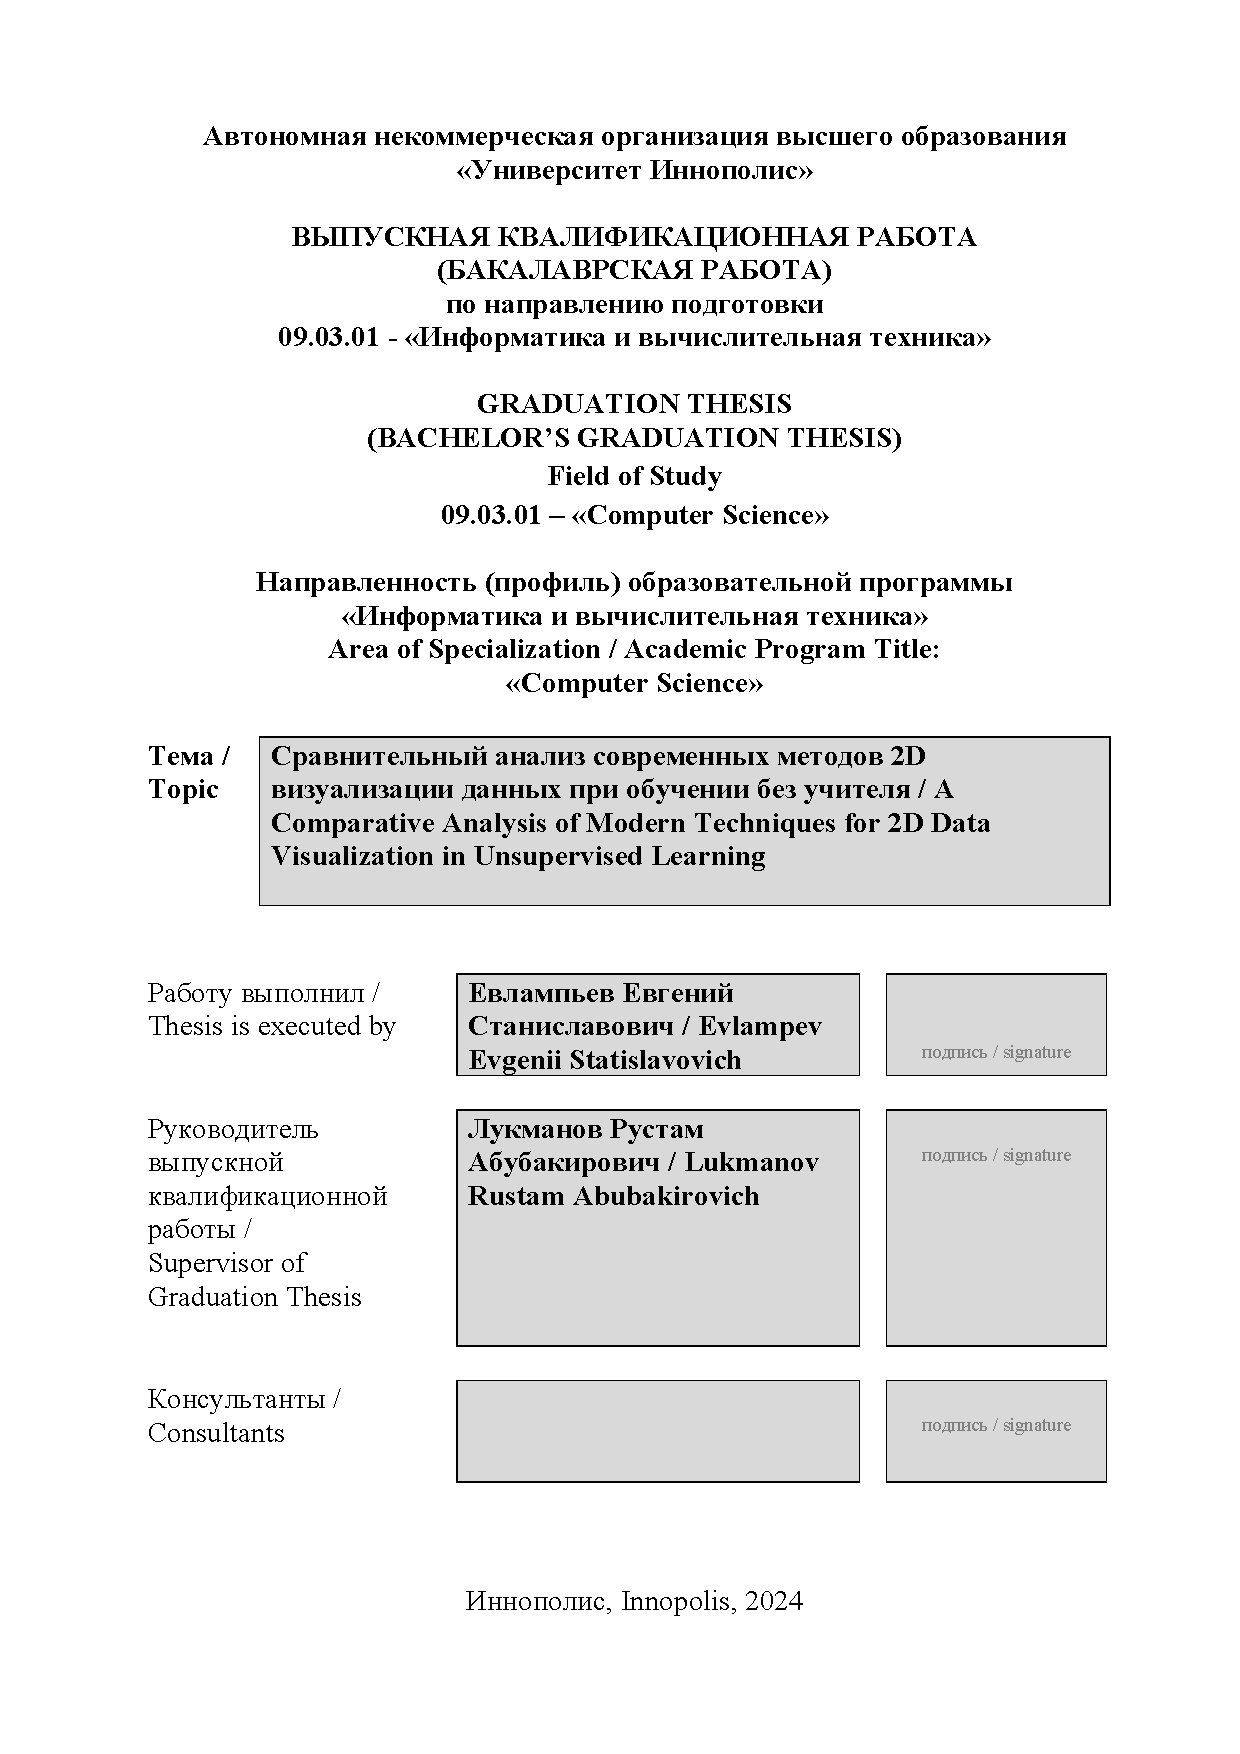
\includepdf[pages=-, offset={25mm, -25mm}, keepaspectratio]{title.pdf}
\tableofcontents
\listoftables
\listoffigures
% \newpage


\begin{abstract}

Modern datasets nowadays contain a significant amount of unlabeled data, presenting challenges in deriving valuable insights. Recent advancements in contrastive learning techniques, such as SimCLR \cite{simclr} and t-SimCNE \cite{tsimcne}, have demonstrated efficacy in this context, particularly for visualizing large datasets and extracting meaningful insights. Despite their effectiveness, these methods often struggle with the requirements for large batch sizes and extensive computational resources, and they may fail to provide clear and distinct 2D visualizations without using GPUs.

To address these limitations, this thesis introduces optimization techniques, specifically AUC-CL and Hard Negative Sampling, to enhance the existing t-SimCNE framework. We conducted a comparative analysis of the modified algorithm, assessing its effectiveness through 2D graphical representations and evaluating its performance across various batch sizes using the k-nearest neighbors (k-NN) classifier. As a result, our enhanced algorithm can make clear visualizations with smaller batch sizes.

For more details and to access to the code you can visit my \href{https://github.com/Evgeneugene/thesis}{GitHub repository}.

\end{abstract}
\setcounter{page}{7}
% set manually the number, from which Chapter 1 starts!
% Why do we put 7 in this case?
% Title page - page 1
% Contents - page 2, page 3
% List of tables - page 4
% List of figures - page 5
% Abstract - page 6
% Chapter 1 - page 7
% In your thesis the counter number can be different, please count carefully and insert the corresponding number.

% \chapter{Introduction}
\label{chap:intro}
\chaptermark{Optional running chapter heading}

\section{Background}
A large amount of data generated today is unlabeled, which complicates the extraction of useful information. Contrastive learning, a type of unsupervised learning, has been effective in leveraging such data, particularly in areas where labeled data is scarce or expensive to obtain. Existing frameworks like SimCLR \cite{simclr} and Momentum Contrast (MoCo) \cite{moco} have shown potential but often struggle with large batch sizes and hyperparameter sensitivity.

Current methods face limitations with scalability and robustness, especially when applied to complex datasets with varying characteristics. These issues highlight the need for more adaptable and efficient learning models.

\section{Research Questions}
This thesis conducts a comparative analysis of modern techniques for 2D data visualization within the framework of unsupervised learning. It examines whether integrating the Area Under the Curve (AUC) metric \cite{sharma2023auc} and Hard Negative Sampling \cite{robinson2020contrastive} with contrastive learning frameworks can address their known limitations and improve their performance across diverse datasets.

\section{Experimental Approach}
The research employs a comparative experimental design using different datasets to evaluate the performance of enhanced contrastive learning methods against traditional approaches. The focus is on accuracy and robustness in visualizing data.

\section{Results and Conclusions}
Results show that adding the AUC metric to contrastive learning frameworks increases their robustness, particularly in limited-resource settings. Also, the adapted framework, t-SimCNE with AUC-CL, provides more clear and interpretable visual representations.

These improvements are significant for data analysis in areas with limited labeled data, potentially improving decision-making and advancing research in various fields.

\section{Thesis Structure}
The structure of our paper is as follows:

\begin{itemize}
    \item Chapter 2: Literature Review – Reviews theoretical background and previous research in unsupervised and contrastive learning.
    \item Chapter 3: Methodology – Describes the experimental methodologies, data sources, and specific frameworks used.
    \item Chapter 4: Results and Analysis – Discusses the experimental results and analyzes the findings.
    \item Chapter 5: Discussion – Interprets the results, discusses implications and limitations, and suggests future research directions.
    \item Chapter 6: Conclusion – Summarizes the study's findings and contributions and outlines future research possibilities.
\end{itemize}
\chapter{Literature Review}
\label{chap:lr}
\chaptermark{Second Chapter Heading}

This chapter is devoted to a review of the literature, which is fundamental for solving the tasks set in our study. The focus is on the use of unsupervised contrastive learning methods to extract features from various datasets, for example, in medicine. 

Section I describes the principles of contrastive learning, its application in areas with limited labeled data. Section II covers the main methods for dimensionality reduction and visualization of high-dimensional data.

\section{Unsupervised Contrastive Learning Approaches}
Contrastive learning is a deep learning technique that is able to derive meaningful representations from data without relying on labels. It focuses on contrasting positive and negative sample pairs and can be used for any type of data, given appropriate augmentations exist.

\subsection{Foundations and Methodological Innovations}

In their work on SimCLR, Chen et al. \cite{tsimcne} described an algorithm for effective contrastive learning and further visualization of data in 2D. SimCLR generates augmented versions of one image, treating them as "positive" pairs and other images as "negative" pairs. Then, the model learns to combine the features of positive pairs and separate the features of negative pairs in the embedding space: a basic neural network extracts elements from images, and then a projection head maps these elements to the space where contrast loss is applied. The focus on different augmentation strategies helps the model to remember the important characteristics needed to understand complex medical images. In addition, using many images increases the number of negative examples, increasing the model's ability to distinguish between different images.

The Momentum Contrast (MoCo) framework by He et al. \cite{moco} further advances the field by introducing a dynamic queue of representations and a momentum-updated encoder. They offer the solution to problems related to time variability and diversity of patient medical data sets. Similarly, a study by BYOL by Grill et al. \cite{byol} gets rid of the need for explicit negative indicators by implementing a new approach that works well with different sets of medical data.

The work by Azizi et al. \cite{azizi} focuses on using large-scale self-supervised models for medical image classification. It shows how big self-learning models can help better use the vast number of medical images that do not have labels and improve and automate medical diagnosis tools.

Sharma et al. \cite{sharma2023auc} addressed the limitations associated with large batch sizes in contrastive learning. They introduced the AUC-Contrastive Learning (AUC-CL) framework, which integrates the area under the ROC curve (AUC) maximization with contrastive learning principles. This approach reduces the dependency on large batch sizes, a common challenge in self-supervised learning frameworks such as SimCLR and MoCo.

\section{Dimensionality reduction for visualisation}

This section explores several pivotal algorithms that have significantly contributed to the field, particularly in the context of 2D visualization of datasets.

One of the foundational techniques in dimensionality reduction is the Locally Linear Embedding (LLE), introduced by Roweis and Saul \cite{roweis2000nonlinear}. LLE is a method of studying the structure of the data that focuses on keeping local groupings unchanged, which is really useful when working with confusing or distorted data. However, LINE may not always be useful for understanding the general layout of data, which may make it less useful for tasks that require a complete overview of the dataset."

Building on the concept of neighborhood preservation, Stochastic Neighbor Embedding (SNE), developed by Hinton and Roweis (2003) \cite{hinton2002stochastic}, introduced a probabilistic framework for dimensionality reduction. SNE aims to maintain similarities between pairs in a low-dimensional space, producing the visualization of clusters or groups within the data. Despite its strengths, SNE's cost function is difficult to optimize, and the algorithm is prone to a "crowding problem," where dissimilar data points collapse onto each other in the reduced space.

To address these limitations, t-SNE (t-distributed Stochastic Neighbor Embedding), as proposed by van der Maaten and Hinton (2008) \cite {van2008visualizing}, uses a t-distribution to measure similarities in the low-dimensional space. This adjustment solves the crowding problem and has made t-SNE a popular choice for visualizing complex datasets. Nevertheless, t-SNE's computational complexity and tendency to form arbitrary clusters due to its sensitivity to hyperparameters can be problematic, especially when interpreting the results scientifically.

In response to the scalability and interpretability challenges of t-SNE, UMAP (Uniform Manifold Approximation and Projection), introduced by McInnes et al. (2018) \cite{mcinnes2018umap}, offers an alternative. UMAP reduces computational time and better preserves the global structure of the data, making a more interpretable mapping from high-dimensional to low-dimensional space.

LargeVis by Tang et al. \cite{tang2016visualizing} and TriMap by Amid and Warmuth \cite {amid2019trimap} further advance in the field, introducing new approaches to balance the preservation of local and global data structures. LargeVis, for example, succeded in handling very large datasets through its efficient neighborhood selection algorithm. TriMap, on the other hand, uses a triplet-based loss function to maintain global relationships.

Parametric mappings is an important development that makes these visualization techniques more adaptable to new data points. Van der Maaten explored this idea \cite{van2009learning} in the context of t-SNE and produced a solution that allows embedding out-of-sample points without re-running the entire algorithm. This parametric approach is promising for real-time data analysis and interactive visualization applications, although it can sometimes sacrifice the detailed structure obtained by nonparametric methods.
\chapter{Methodology}

This chapter outlines the methodologies employed in our study. In Section I we begin with a discussion of the datasets used. In Section II, we explore the application and customization of SimCLR and t-SimCNE. In Section III we describe our hard negative sampling approach.
Section IV introduces the AUC-CL framework we used to incorporate the Area under the ROC curve metric.

\section{Datasets}
\subsection{CIFAR-10}
The CIFAR-10 dataset \cite{cifar10} comprises 60,000 images in 32x32 resolution, each in full color, and is distributed evenly across 10 classes. This dataset is commonly used for benchmarking image recognition algorithms, providing a diverse range of object classes to test the robustness and generalizability of models.


\subsection{MedMNIST}
Medmnist \cite{medmnist} is a standardized collection of medical image datasets for deep learning benchmarks. It includes different medical imaging data, such as dermatological, radiological, and hematological images. We used Dermamnist and Bloodmnist datasets.

Dermamnist dataset contains 10,015 dermatological images, each resized to 28x28 pixels in grayscale. These images are categorized into seven classes. This subset of Medmnist is designed for the task of skin disease classification.

Bloodmnist dataset includes 17,092 microscopic images of blood cells, standardized to 28x28 pixel grayscale images. These images are categorized into eight types. Bloodmnist facilitates the training of models for the classification of blood cells, aiding in the diagnosis of hematological diseases.

\subsection{Leukemia}
The Leukemia dataset \cite{leukemia} consists of microscopic images of white blood cells sourced from patients, including those diagnosed with leukemia. The original resolution is 224 x 224, so we downscaled these images to 28 x 28 to align with the MedMNIST standards.


\section{SimCLR algorithm}
SimCLR (Simple Contrastive Learning of Representations) is a self-supervised learning framework designed to learn visual representations without requiring labeled data. The core idea of SimCLR is to maximize agreement between differently augmented views of the same image via a contrastive loss. This method operates in several steps:

\subsection{Data Augmentation}
Each image in the dataset is transformed twice using random data augmentation techniques such as cropping, resizing, color distortion, and Gaussian blurring to generate two correlated views, denoted as positive pairs. 

\subsection{Feature Extraction}
Both augmented images are then fed into a shared convolutional neural network to extract features.

\subsection{Projection Head}
The representations are then passed through a projection head, which is a small feed-forward neural network, to obtain the final representations used in the contrastive loss calculation.

\subsection{Contrastive Loss}
SimCLR utilizes the contrastive loss function known as normalized temperature-scaled cross-entropy loss (NT-Xent). The loss function for a positive pair of examples $(i, j)$ is given by:

\begin{equation}
\ell(i, j) = -\log \frac{\exp(\text{sim}(z_i, z_j) / \tau)}{\sum_{k=1}^{2N} \mathbf{1}_{[k \neq i]} \exp(\text{sim}(z_i, z_k) / \tau)}
\end{equation}

where $\text{sim}(u, v) = \frac{u^\top v}{\|u\| \|v\|}$ denotes the cosine similarity between $u$ and $v$, $\tau$ is a temperature scaling parameter, and $N$ is the batch size. The indicator function $\mathbf{1}_{[k \neq i]}$ is 1 iff $k \neq i$ and ensures that a sample does not form a negative pair with itself.

This loss function encourages representations of positive pairs to be closer to each other while pushing representations of negative pairs (different images) apart in the embedding space.

\section{Extension of SimCLR with t-SimCNE}
\subsection{Overview}
We used t-SimCNE (t-distributed Simultaneous Contrastive Neighbor Embedding) to extend the SimCLR framework by optimizing direct mapping from the high-dimensional pixel space to a two-dimensional embedding space. This method is designed to produce meaningful and interpretable visualizations of image datasets by preserving semantic relationships within the data.

t-SimCNE modifies the typical contrastive learning approach by using a two-dimensional output directly during the training phase rather than using the high-dimensional outputs typical of models like SimCLR. This approach allows for immediate data visualization without additional dimensionality reduction steps.

\begin{figure}[hbt]
\centering
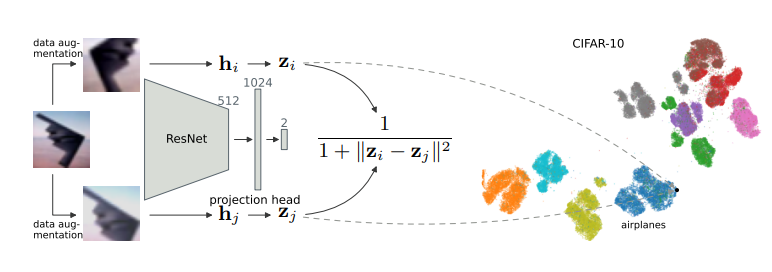
\includegraphics[width=\textwidth]{figs/tsimcne_architecture.png}
\caption{
t-SimCNE algorithm \cite{tsimcne}.
}
\label{fig:secex}
\end{figure}

\subsection{t-SimCNE Loss Function}
The t-SimCNE modifies the contrastive loss function by incorporating the Cauchy kernel, which is particularly effective for handling the crowding problem at lower dimensions. The loss function is given by:

\begin{equation}
\mathcal{L}(i, j) = -\log \left(\frac{\frac{1}{1 + \|z_i - z_j\|^2}}{\sum_{k=1}^{2N} \mathbf{1}_{[k \neq i]} \frac{1}{1 + \|z_i - z_k\|^2}}\right)
\end{equation}

Here, $z_i$ and $z_j$ are the two-dimensional embeddings of two different augmented views of the same image, and $\|z_i - z_j\|^2$ represents the squared Euclidean distance between the embeddings $z_i$ and $z_j$. The temperature parameter traditionally used in the softmax function is implicit in the normalization by the Cauchy kernel, and $N$ is the batch size used during training.


\subsection{Training Strategy}
t-SimCNE involves several key stages in training:
\begin{itemize}
    \item Pre-training in a higher dimensional space (typically 128D) to stabilize the learning of useful features.
    \item Fine-tuning the network to produce 2D outputs for direct visualization.
    \item An additional fine-tuning phase over the entire network to refine the embeddings and improve the visualization quality.
\end{itemize}


\section{Visualization Algorithms}
We tested different visualization algorithms to prove that t-SimCNE is the best one.

\subsection{Standalone t-SNE}

t-SNE is an algorithm used to visualize high-dimensional data in two or three dimensions. The algorithm works by converting similarities between data points to joint probabilities and minimizing the Kullback-Leibler divergence between the joint probabilities of the low-dimensional embedding and the high-dimensional data.

t-SNE starts by calculating probabilities in the high-dimensional space that are related to the similarity of data points:
\[
p_{j|i} = \frac{\exp(-\|x_i - x_j\|^2 / 2\sigma_i^2)}{\sum_{k \neq i} \exp(-\|x_i - x_k\|^2 / 2\sigma_i^2)}
\]
where \(p_{j|i}\) represents the probability that point \(x_j\) would be picked as a neighbor of point \(x_i\) under a Gaussian centered at \(x_i\) with variance \(\sigma_i^2\).

In the low-dimensional space, t-SNE defines a similar probability but using a Student-t distribution:
\[
q_{ij} = \frac{(1 + \|y_i - y_j\|^2)^{-1}}{\sum_{k \neq l} (1 + \|y_k - y_l\|^2)^{-1}}
\]
where \(y_i\) and \(y_j\) are the embeddings of points \(x_i\) and \(x_j\) in the low-dimensional space.

The goal of t-SNE is to minimize the difference between these probability distributions:
\[
C = \sum_i \sum_j p_{ij} \log\left(\frac{p_{ij}}{q_{ij}}\right)
\]

\subsection{t-SimCNE}
Unlike traditional dimensionality reduction methods, t-SimCNE integrates visualization directly into the learning process, turning complex image datasets into two-dimensional data without the need for postprocessing. This method addresses the limitations of t-SNE and UMAP by preserving both local and global structures within the data.

\subsection{t-SNE with SimCLR}
When combined with SimCLR, t-SNE is used to further process the 128-dimensional outputs generated by SimCLR. This method helps in identifying how similar or different the images are, simplifying the complexity of high-dimensional data for easier analysis. This integration provides a practical way to see and understand the natural groupings within a dataset.


\section{Hard Negative Sampling}
We integrated hard negative sampling into the t-SimCNE framework to refine the model's ability to differentiate between similar yet distinct image features effectively. This method addresses the challenge of selecting informative negatives without supervision.

\subsubsection{Importance}
Hard negative samples are those data points that are close to the anchor point in the embedding space but have different classes. By emphasizing these hard negatives, t-SimCNE can generate embeddings that more accurately reflect the underlying data structure and improve the separation between different classes in complex datasets.

\subsubsection{Mathematical Formulation}
The selection of hard negatives in the t-SimCNE is guided by a sampling distribution, which prefers negatives whose representations are very similar to the anchor, providing a stronger gradient during training. This can be mathematically represented as:

\begin{equation}
q_{\beta}(x^-) \propto \exp(\beta \cdot f(x)^T f(x^-)) \cdot p(x^-)
\end{equation}

where $f(x)$ and $f(x^-)$ are the features of the anchor and negative samples, respectively, $\beta$ is a parameter controlling the "hardness" of the negatives, and $p(x^-)$ is the probability distribution of the negatives.

\subsubsection{Implementation in t-SimCNE}
To incorporate hard negative sampling into t-SimCNE, we adjust and weigh the selected hard negatives more heavily during the contrastive loss computation. This adjustment helps focus on critical features for distinguishing between similar yet categorically different images.

\section{AUC-CL Framework}
The AUC-Contrastive Learning (AUC-CL) framework further enhances our contrastive learning approach by integrating the Area under the receiver operating characteristic (ROC) curve (AUC) maximization into the learning objective. This method addresses the limitations of contrastive learning related to batch size sensitivity and optimization biases.

\subsection{Motivation and Definition}
In contrastive learning, the choice of batch size can significantly impact performance due to the biased estimation of gradients from small sample sizes. AUC-CL proposes to resolve this using the AUC metric, which evaluates the probability that a randomly chosen positive instance is ranked higher than a randomly chosen negative instance. The goal is to maximize this probability, ensuring that positive pairs have higher similarity scores than negative pairs.

\subsection{AUC Maximization}
The Area Under the Receiver Operating Characteristic Curve (AUC-ROC) is a measure of the ability of a classifier to distinguish between classes. For a binary classifier \( h_w \) parameterized by \( w \) with labeled samples \( \{x, x'\} \) where \( y = 1 \) and \( y' = -1 \) represent positive and negative classes respectively, the AUC is defined as:

\[
AUC(w) = P(h_w(x) \geq h_w(x') \mid y = 1, y' = -1)
\]

This equation states that the AUC is the probability that a randomly chosen positive example is scored higher by the classifier than a randomly chosen negative example.

The direct computation of AUC involves considering all possible pairs of positive and negative samples. For a dataset with \( N \) samples, if the numbers of positive and negative samples are approximately equal, this leads to \( O(N^2) \) complexity. This is because each positive sample is compared against each negative sample to compute the AUC, which becomes computationally intensive for large datasets.

To address the computational challenge, we reformulate it using a square loss function:

\[
L(w) = E\left[(1 - h_w(x) + h_w(x'))^2 \mid y = 1, y' = -1\right]
\]

This loss function simplifies the optimization problem by transforming the original probability comparison into a squared error term, which is easier to handle computationally. The expectation \( E \) averages over all positive-negative pairs, but the squared term allows the gradient of the loss with respect to the parameters \( w \) to be computed more efficiently. 

Minimizing the previous equation, we get the final loss function.

\subsection{AUC-CL Loss Function}
The AUC-CL framework is as follows:
\[
L'_s(w, b; x_i, A, A', B_i) = A_1 + A_2 + A_3
\]
where
- \(A_1\): Positive pair term, penalizing the distance between embeddings of the same image under different augmentations.
  \[
  A_1 = \left[ (\text{sim}(i, i+) - a)^2 \right] \text{ where } y_{ii+} = 1
  \]

- \(A_2\): Negative pair term, penalizing the closeness between embeddings of different images.
  \[
  A_2 = \sum_{j \in B_i} \left[ (\text{sim}(i, j) - b)^2 \right] \text{ where } y_{ij-} = 1
  \]

- \(A_3\): Regularization term to balance the contribution of positive and negative pairs.
  \[
  A_3 = \left\{ 2\alpha \left[ 1 - \text{sim}(i, i+) + \sum_{j \in B_i} \text{sim}(i, j) \right] - \alpha^2 \right\}
  \]

The variables are:
- \(w, b\): Parameters to optimize.
- \(x_i\): Training sample.
- \(A, A'\): Augmentation functions.
- \(B_i\): Batch subset excluding \(x_i\).
- \(\text{sim}(i, j)\): Similarity measure, typically cosine similarity.
- \(a, b\): Baseline similarities for positive and negative pairs.
- \(\alpha\): Scaling factor for the regularization term.


\begin{figure}[hbt]
\centering
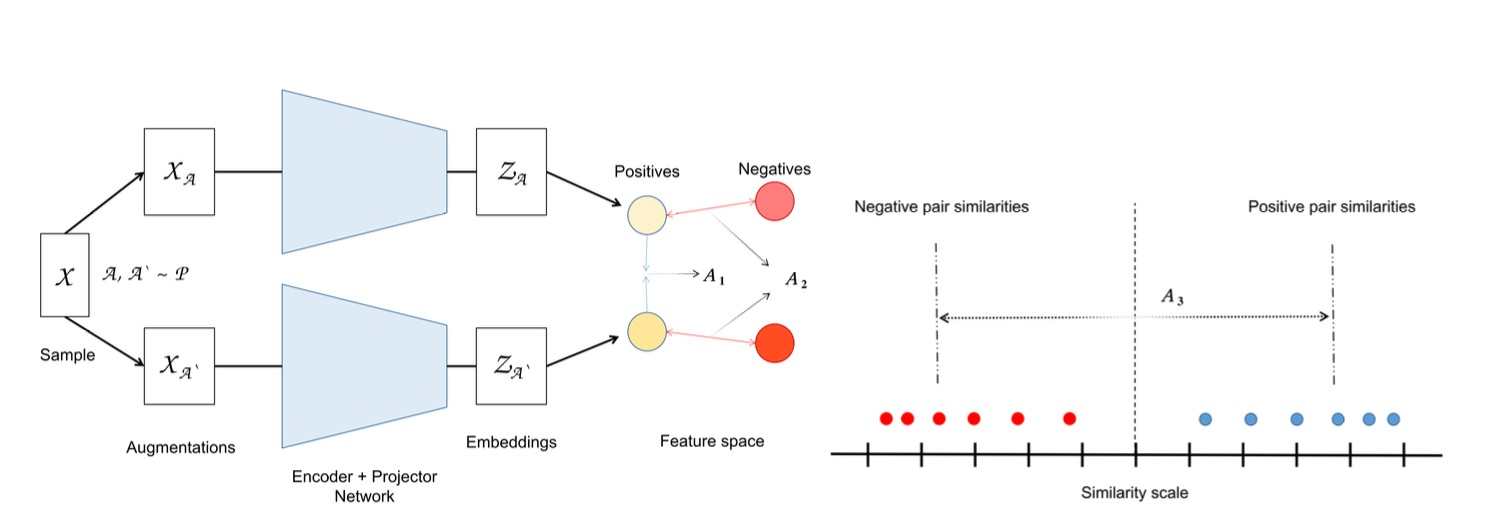
\includegraphics[width=\textwidth]{figs/auc-cl.png}
\caption{
AUC-CL schema \cite{sharma2023auc}.
}
\label{fig:secex}
\end{figure}

\subsection{Optimization and Robustness}
The integration of the AUC into the contrastive learning framework helps stabilize the training under conditions of limited computational resources or smaller batch sizes. This stability is due to the unbiased nature of the gradient updates provided by the AUC component, which does not suffer from the large variance typically seen with small batches in traditional contrastive learning setups.

% \chapter{Implementation}

In the this chapter, we delve into practical exploration of the t-SimCNE framework, a novel method designed to enable unsupervised visualization of image datasets via contrastive learning. During implementatioin we relied on the code from the t-SimCNE GitHub repository, which provided the foundational codebase for this study.

\section{Training Settings}

Following the steps of Böhm et al. \cite{tsimcne}, we reproduced the training environment and model's settings in a similar way.

\subsection{Model Architecture}

The model utilizes a ResNet architecture, specifically a ResNet18. After feature extraction through the ResNet backbone, the model employs a fully-connected projection head.

\subsection{Pre-training}
The model is first pre-trained to output 128-dimensional embeddings for 100 epochs. This stage uses the full architecture, including the backbone and the projection head, to stabilize the feature space before reducing dimensionality.

\subsection{Fine-tuning}
After pre-training, the model undergoes a fine-tuning process where only the 2D readout layer is initially fine-tuned for 10 epochs to adjust to the lower-dimensional output. Subsequently, the entire network is fine-tuned for an additional 40 epochs to refine the 2D embeddings.

\subsection{Optimizer}
Stochastic Gradient Descent (SGD) with momentum (set to 0.9) is used. This optimizer is effective for navigating the complex landscapes of high-dimensional data typical of deep learning tasks.

\subsection{Learning Rate}
The initial learning rate is set to 0.12, scaled by the batch size relative to 256. This learning rate warm-ups over the first ten epochs, after which it follows a cosine annealing schedule down to zero. 

\subsection{Data Augmentation}
Essential to the contrastive learning approach, data augmentations such as random cropping and flipping are applied to generate diverse views of the same image, enhancing the model's ability to generalize from unlabelled data.

\section{Reproducing results}

My implementation began with the CIFAR-10 dataset, a standard benchmark in the machine learning community for evaluating algorithmic advancements in image recognition. The CIFAR-10 dataset consists of 60,000 32x32 color images in 10 different classes. Given the limitations of my computational resources, particularly GPU availability, we made a decision to adjust the training epochs from the 1000 outlined in the original experiments to ~150 epochs for my trials. This decision was influenced by the computational expense associated with the original settings, where one experiment could consume approximately 20 hours of GPU time. As a result, we reproduced the model's weights and data visualizations in the original t-SimCNE paper \cite{tsimcne}.

\begin{figure}[hbt]
\centering
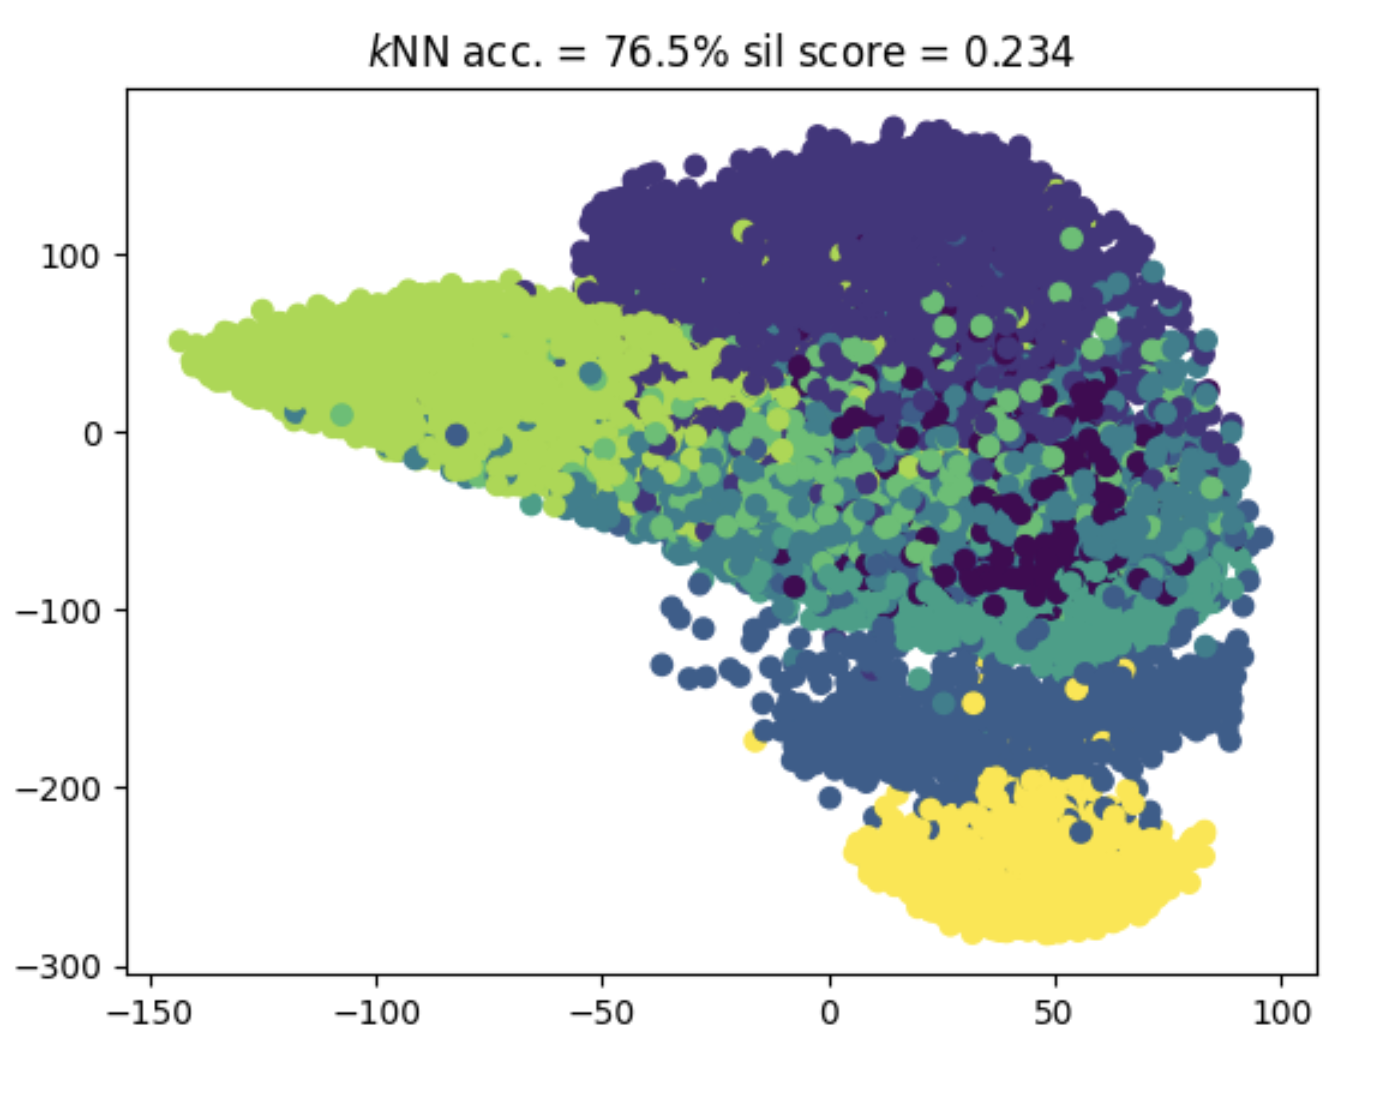
\includegraphics[width=\textwidth]{figs/cifar-10-tsimcne-2.png}
\caption{The visualization of the CIFAR-10 dataset using t-SimCNE with 150 epochs. Each color represents a separate class}
\label{fig:secex}
\end{figure}

\section{Hard Negative Sampling}
To amplify the contrastive learning signal by focusing on difficult yet informative negative examples, we integrated a hard negative sampling strategy into the existing InfoNCE loss function. The adapted InfoNCE loss, which we implemented as InfoNCECauchyHardNegative, has a temperature parameter and a beta parameter. The temperature controls the scale of the distribution, affecting the separation between similar and dissimilar points, while the beta parameter adjusts the emphasis on harder negatives.


\section{AUC-CL}

Besides the Hard Negative Sampling approach, we tested the loss function of the AUC-CL algorithm. It the same sense as previously, it calculates the similarity between features within each group and across the two groups using a similarity function that emphasizes features that are close in the feature space. This similarity function is fine-tuned with a temperature parameter, which helps control the sensitivity of the function to differences between features.

For the features that are similar, the loss function encourages the model to recognize and enhance these similarities, aiming to align similar features more closely. For the dissimilar feature pairs (those within the same group), the model is encouraged to distinguish between them more clearly. This is achieved by adjusting the emphasis on harder negative examples. This emphasis is controlled by another parameter in the loss function, which scales the impact of these harder negatives.

Furthermore, the function includes a dynamic adjustment mechanism, which regulates the contribution of each type of feature pair (similar and dissimilar) to the overall loss. This adjustment ensures that the model balances its attention between pulling similar items closer and pushing dissimilar items further apart in the feature space.

\section{Experimentation with Diverse Datasets}

To evaluate the efficacy and versatility of the modified loss functions, we conducted a series of experiments across multiple datasets. The primary objective was to assess how the modified t-SimCNE and t-SNE with SimCLR, as well as standalone t-SNE, perform in terms of the quality of visualization and the ability to capture meaningful class separations in different contexts. The datasets chosen for this study were CIFAR-10, Leukemia, Bloodmnist, and Dermamnist, each offering unique challenges and characteristics.

\subsection{Visualization Techniques}
\begin{enumerate}
\item {Standalone t-SNE}: As a baseline, standalone t-SNE was used to visualize the datasets without the influence of contrastive learning.
For each dataset, we applied three different visualization techniques:
\item {t-SNE with SimCLR}: We also explored a hybrid approach where t-SNE is applied to embeddings generated by SimCLR.
\item {t-SimCNE}: Our primary focus was on the modified t-SimCNE, which incorporates the newly adapted loss functions.
\end{enumerate}

\subsection{Implementation Details}
We adapted to the computational constraints and specific challenges posed by each dataset. Given the varying complexity and size of the datasets, the number of training epochs, batch sizes, and specific parameters for each visualization technique were tuned accordingly.

% \setcounter{chapter}{4} % This makes the next chapter 5
% \chapter{Results and Evaluation}
\label{chap:eval}

This chapter presents the results of the experiments conducted using diverse datasets and visualization techniques. The primary focus was to evaluate the effectiveness of the modified t-SimCNE, the hybrid t-SNE with SimCLR, and the standalone t-SNE. The chapter also examines the impact of different loss functions on the quality of data visualization and the ability to discern class separations.

\section{Visualization Outcomes}

Each visualization method was applied to CIFAR-10, Leukemia, Bloodmnist, and Dermamnist datasets:

\begin{figure}[hbt]
\centering
\includegraphics[width=\textwidth]{figs/toy_datasets_tsimcne.png}
\caption{2D embeddings of the datasets using standard t-SimCNE with 150 epochs (which is considered small)
}
\label{fig:med_tsimcne}
\end{figure}

\begin{figure}[hbt]
\centering
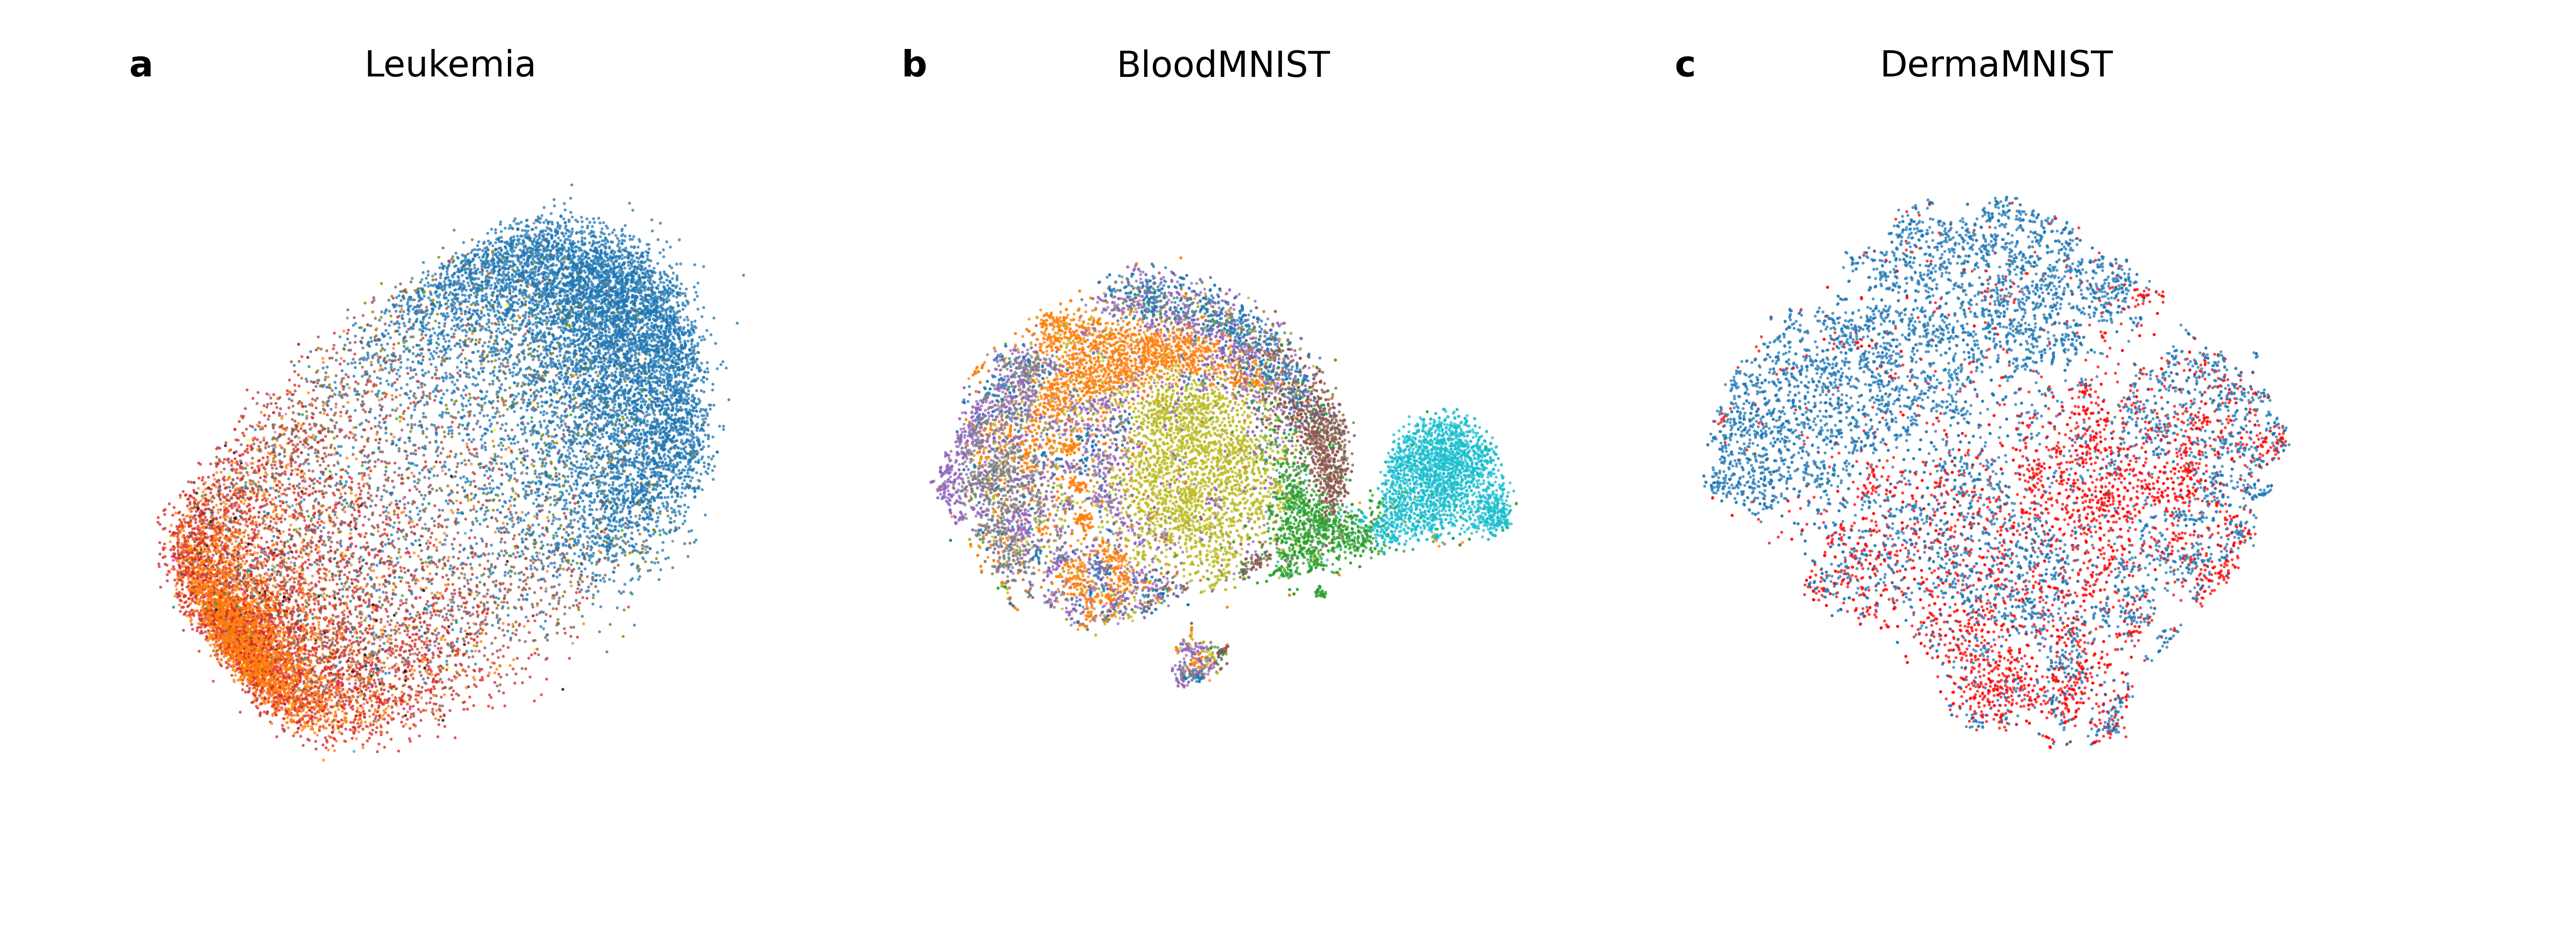
\includegraphics[width=\textwidth]{figs/toy_datasets_tsne.png}
\caption{
2D embeddings of the datasets using t-SNE
}

\label{fig:med_tsne}
\end{figure}

Figure~\ref{fig:med_tsimcne} illustrates the 2D visualizations of learned representations with standard t-SimCNE. It is worth noting that KNN accuracy and overall feature representation quality increases with training, but it requires more computational time and a large number of epochs.

Figure~\ref{fig:med_tsne} illustrates the 2D visualizations with the use of standalone t-SNE without any learning. They may seem to be more accurate visually, discerning the data better, but as Böhm et al. \cite{tsimcne} noted, there are two main problems: 

\begin{itemize}
    \item They don't clearly show details like outliers or different subgroups, making them harder to understand compared to t-SimCNE visualizations
    \item They can't be used to add new images into an already existing visualization, which is something that can be very useful in real-world uses.
\end{itemize}

\begin{figure}[hbt]
\centering
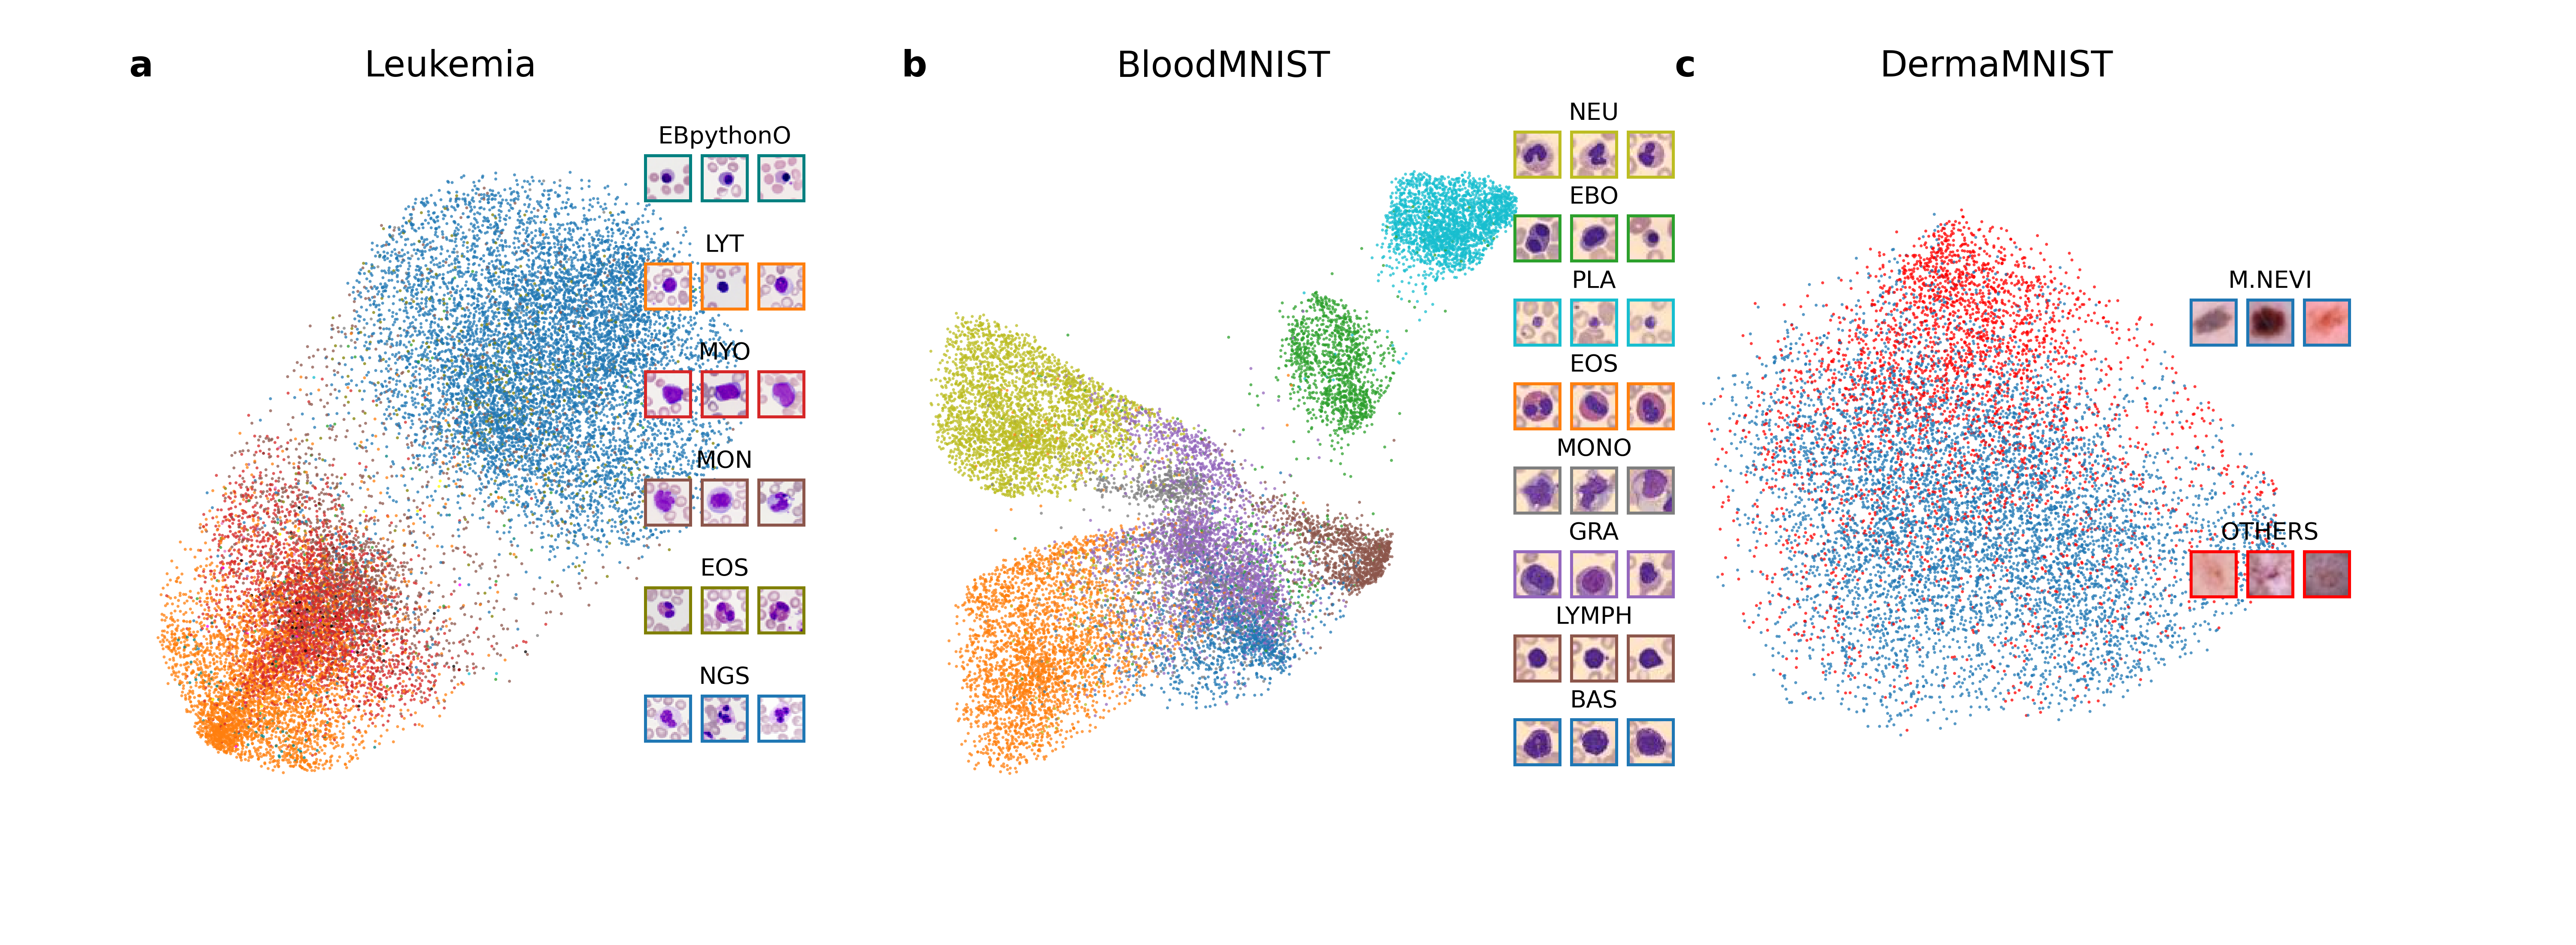
\includegraphics[width=\textwidth]{figs/toy_datasets_long_2.png}
\caption{
2D embeddings of the datasets using our approach with t-SimCNE and AUC-CL
}
\label{fig:tsimcne_auc_cl}
\end{figure}


Unfortunately, our hard negative sampling approach had neither visual nor metrical improvements (Figure~\ref{fig:hardneg}). However, the AUC-CL approach has shown a small rise in performance. Figure~\ref{fig:tsimcne_auc_cl} shows that our implementation of the t-SimCNE algorithm with integration of the AUC-CL approach resulted in a better visual results than both of the previous methods and enhanced ability to discern distinct data clusters more clearly, while using a smaller batch size (256), which requires much less computing power.

\begin{figure}[hbt]
\centering
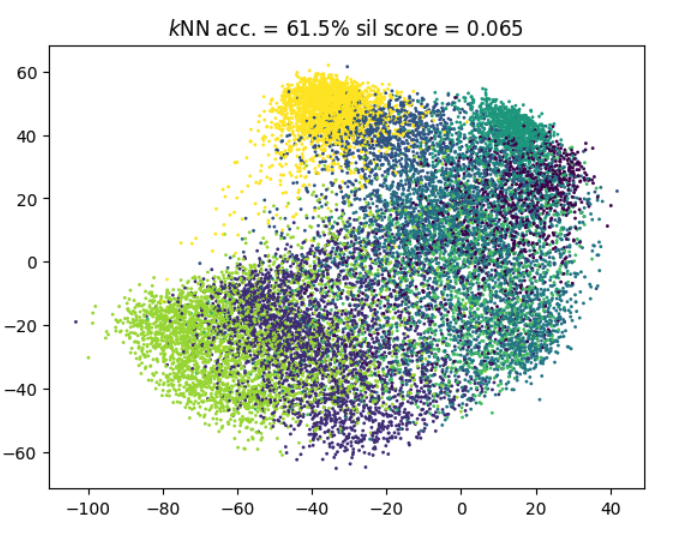
\includegraphics[width=\textwidth]{figs/hardneg.png}
\caption{
Our Hard Negative Sampling approach for CIFAR-10 dataset with 150 epochs.
}
\label{fig:hardneg}
\end{figure}

\subsection{Quantitative Evaluation}

Quantitative metrics were employed to further evaluate the performance of each visualization technique:

\begin{itemize}
    \item {k-NN Classifier}: Used to assess the quality of embeddings by measuring classification accuracy on the low-dimensional data produced by each visualization technique. Results indicate that embeddings from t-SimCNE and t-SNE with SimCLR outperform those from standalone t-SNE.
    \item {Robustness to Batch Size Variations}: Particularly for AUC-CL, we observed minimal loss in accuracy with reduced batch sizes, highlighting its robustness compared to traditional contrastive learning approaches.
\end{itemize}

\begin{figure}[hbt]
\centering
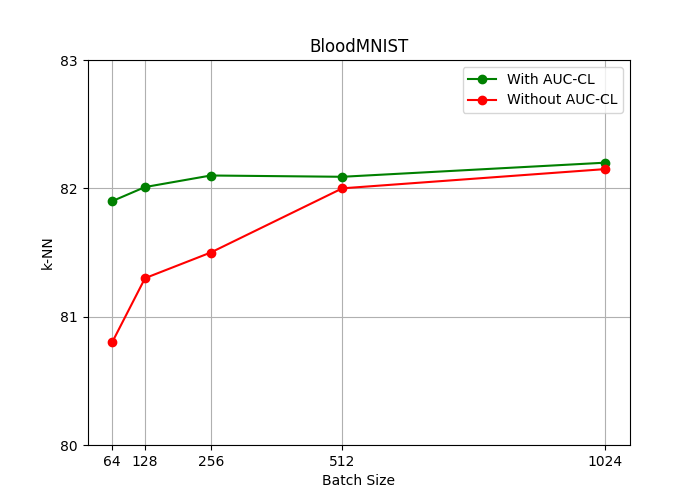
\includegraphics[width=\textwidth]{figs/accuracy_comparison.png}
\caption{
k-NN classifier with different batch sizes using the AUC-CL approach for the BloodMNIST dataset
}
\label{fig:knn_comparison}
\end{figure}


The plot \pic{fig:knn_comparison} shows that the inclusion of AUC-CL in the training process leads to higher k-NN accuracy across all batch sizes. 
Additionally, our method maintains consistent performance across different batch sizes, showing robustness, which can be particularly useful with limited computational resources.




% \chapter{Conclusion}
\label{chap:conclusion}
\section{Summary of Findings}

In  this thesis we implemented various advanced unsupervised learning techniques for 2D data visualization and conducted a comparative analysis. Our study focused primarily on frameworks such as SimCLR, t-SimCNE, and AUC-CL, testing these methodologies across diverse datasets including CIFAR-10, Leukemia, Bloodmnist, and Dermamnist.

The findings of this research underscore several key points:
\begin{enumerate}
    \item {Enhanced Visualization Capabilities:} Among the tested methodologies, t-SimCNE combined with the AUC-CL framework provided superior visualization results while using smaller batch sizes. 
    \item {Robustness to Batch Size Variations:} An important feature of the AUC-CL framework is its robustness against batch size variations, making it suitable for scenarios with computational resource constraints.
    \item {Quantitative Metrics:}  The use of metrics, like k-NN classifier accuracy, confirmed that the embeddings from t-SimCNE augmented with AUC-CL have better quality.
    
\end{enumerate}

\section{Future Work}

Further research can build on the work of this thesis by looking for better ways to handle large amounts of data and improve our algorithms. Additionally, developing tools and hard negative sampling techniques for selecting informative negative examples could enhance these methods. More so, future studies can try using our current solutions on more complex datasets and with more computational power for longer periods, which could help produce much clearer and more clustered visual representations of data. 

\section{Concluding Remarks}

The research conducted for this thesis advances the understanding and application of contrastive learning techniques for 2D data visualization. By developing and implementing robust, resource-efficient strategies, this work contributes to making data visualization techniques more accessible and practical across various domains. The further refinement and adaptation of these methods are important in addressing the evolving challenges within the field of artificial intelligence.
\ldots


%% REFERENCES
\printbibliography[heading=bibintoc,title={Bibliography cited}]

\end{document}